\chapter{Background}

In this chapter we present an overview of the related research with the topic of our thesis. Firstly, we describe how the human brain can acquire new knowledge, the process of retention of information and the retrieval of information from memory. Secondly, we give an overview of the techniques suitable for educational systems with the focus on adaptive learning of facts.

\section{Student Modeling and Memory}

Throughout the last one hundred years, researchers have been trying to figure out the complex cognitive processes in the human brain, which are responsible for our ability to learn~\cite{RichardE.Mayer2010}. Understanding the process of learning can be very helpful in education and educational systems where we wish to improve the student's representation. This is useful if we want to adapt our system to the needs and knowledge of individual students practicing a particular domain (e.g. the knowledge of animals, Japanese vocabulary or geography). The construction of a quantitative representation, called a \textit{student model}, is known as \textit{student modeling}~\cite{Sison1998}.

The Greek philosopher and mathematician Plato compared human mind to an aviary in which each bird represented a memory~\cite{MichaelW.Eysenck2008}. Today, we have a much better intuition on the human biological storage -- the hardware responsible for the storage and organization of data in modern computers. This analogy of computer data storage is much better than the one Plato used and it seems to be very close and accurate depiction of the human memory.

So far, we haven't mentioned learning, which is very closely related to memory and to the topic of our thesis. Learning leads to the creation of memory. The study of learning and memory can be divided even further when we realize that we need some way to observe what the students know by experiments. This section is thus explained in three parts:

\begin{itemize}
  \item Learning
  \item Memory
  \item Performance
\end{itemize}

This distinction is not very important, however, it can help the reader better understand the underlying problem discussed in our thesis, the connection between computer science and psychology. In a book released by a professor of psychology at the University of California Richard~E.~Mayer, the science of learning is organized differently, that is into the following three components:

\begin{itemize}
  \item The science of learning
  \item The science of instruction
  \item The science of assessment
\end{itemize}

All of these components are to some extent related to our research. However, the science of learning is the most related since it concerns human memory and learning. The science of instruction is about the manipulation of the student's environment in order to foster learning, it's the scientific study of how to help people learn. In educational systems, this is usually done by incorporating \textit{instructional policies}, the strategies or a set of instructions that help students maintain engagement and increase the amount gained knowledge in one session. Instructional policies guide students during learning by e.g. the selection of appropriate questions or the number of options in multiple-choice tests. Lastly, the science of assessment seeks to determine what people know, which is important so that we are able to quantify the effectiveness of different instructional methods~\cite{RichardE.Mayer2010}.

\subsection{Learning}

\begin{figure}[htbp]
  \centering
  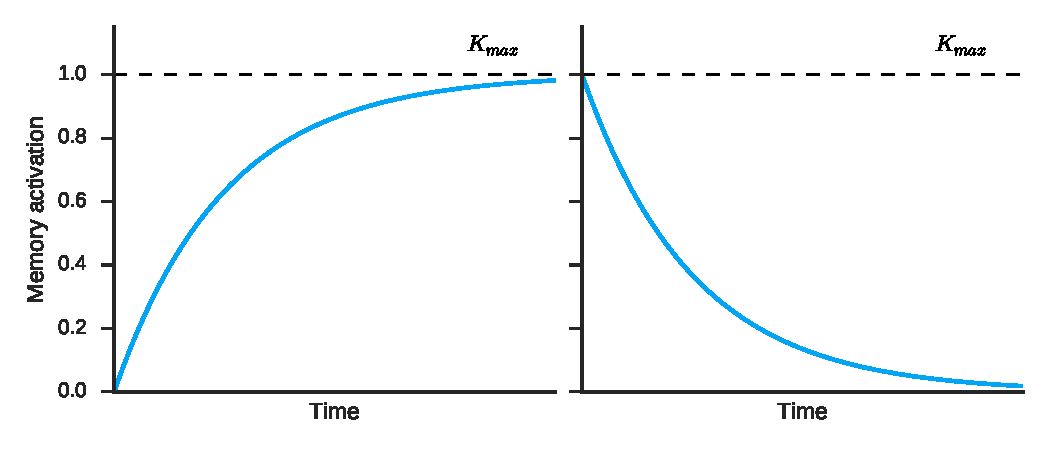
\includegraphics[width=\textwidth]{img/learning-forgetting-curves}
  \caption{Learning curve (left) and forgetting curve (right).}
  \label{fig:learning-forgetting-curves}
\end{figure}

Richard E. Mayer formulated learning as a change in what the student knows caused by the student's experience~\cite{RichardE.Mayer2010}. More specifically, learning is the process of encoding, modifying and reinforcing information~\cite{Lewis}. For example the encoding of the location of Portugal can be seen as learning the shape of the country, its neighbor Spain and the surrounding ocean.

A learning curve is the rate of the student's progress in gaining new skill or knowledge by experience in the environment (e.g. by participating in a discussion, reading a book or riding a bike). Generally, the speed of learning is proportional to the product of amount learned and amount to yet learn. This can be written mathematically:

\begin{equation} \label{learning-differential}
  \frac{dK}{dt} = a \cdot (K_{max} - K)
\end{equation}

The coefficient $a$ in the Equeation~\ref{learning-differential} represents the rate of learning. $K$ is the student's knowledge and $K_{max}$ the maximum knowledge possible. Several functions modeling the learning curve were proposed in the past, namely the power law, exponential and hyperbolic function. Most researchers nowadays believe that learning follows the power law~\cite{Klusasek2014}.

In order to model learning we need to be able to measure \textit{memory strength}, which is a measurement of the ability to retrieve an \textit{item} from memory. In our case an item is any information that can be learned. Memory strength can be measured indirectly by observing the following attributes of students when an item is practiced:

\begin{description}[leftmargin=0cm]
  \item[Probability of recall] Probability of the student recalling the practiced item, this can be measured as the fraction of the number of successful recollections and the number of all presentations.
  \item[Latency of recall] Latency of the student when retrieving the practiced item from memory. Latency of recall can be measured by observing the response times of students.
  \item[Savings in relearning] The number of required revisions of the practiced item in order to fully regain its knowledge~\cite{MichaelW.Eysenck2008}.
\end{description}

We can further distinguish the following levels of learning as measured by memory strength (portrayed on Figure~\ref{fig:knowledge-levels}):

\begin{figure}[htbp]
  \centering
  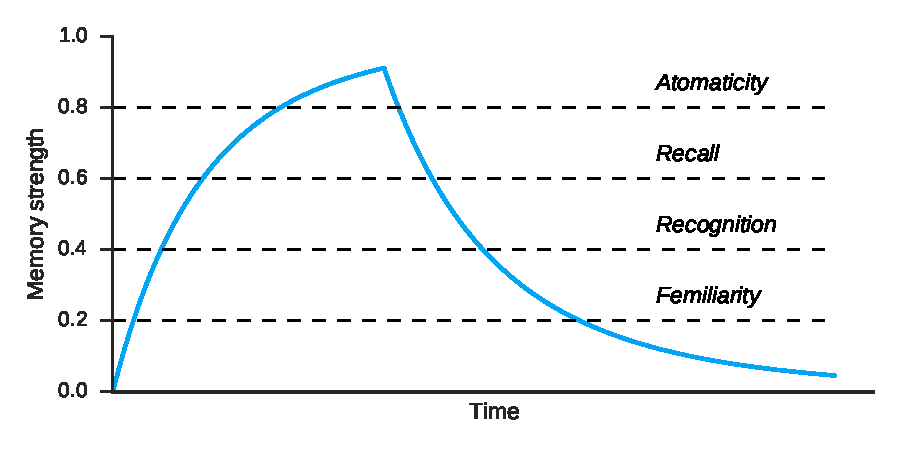
\includegraphics[width=\textwidth]{img/knowledge-levels}
  \caption{Different levels of learning.}
  \label{fig:knowledge-levels}
\end{figure}

\begin{description}[leftmargin=0cm]
  \item[Familiarity] The student has feeling they knew the item in the past but cannot remember anymore.
  \item[Recognition] The student recognized the item when presented multiple-choice options but couldn't remember otherwise.
  \item[Recall] The student is able to recall the item with some effort. Note that in cognitive science we distinguishe \textit{free recall} and \textit{cued recall}. Free recall is the ability to remember an item without any help (e.g. recalling the name of a country), in the case of cued recall, we are given an information which can help us remember (e.g. first letter of the country we are to remember).
  \item[Automaticity] The student recalls the item instantaneously when presented. Note that the level of automaticity can be measured by the latency of recall.
\end{description}

\subsection{Memory}

Memory is the biological storage that retains encoded information, e.g. the location of Portugal. We recognize at least three types of memory (the sensory memory, the short-term memory and the long-term memory) all of which don't retain information permanently and decay with time. The long-term memory decay is called \textit{forgetting} and similarly as learning it respects the power law~\cite{MichaelW.Eysenck2008}.

The effect of forgetting (i.e. loss of information) can be reduced by repetition. Repetition can be massed or spaced, in a massed presentation an item is revised in a short intervals many times over. In contrast, a spaced presentation usually consists of revisions performed across longer periods of time with pauses between presentations. It is well known that a spaced presentation leads to a better memory strength~\cite{RichardE.Mayer2010}. This phenomenon is called the \textit{spacing effect}.

The next matter we shell discuss is the classification of long-term memory by information type. Most importantly we shell distinguish the procedural (knowing how) and declarative (knowing what) memory. The procedural memory is the memory we aren't consciously aware of and which makes humans capable of the acquisition of both the motor and cognitive skills. For example riding a bike or swimming are tasks that are learned and collected as procedural memories. The declarative memory is the conscious knowledge such as the world's countries or the English vocabulary~\cite{MichaelW.Eysenck2008}.

\subsection{Performance}

The performance of students is the determination of what they know. Performance can be estimated from the speed and precision of recall, e.g. by a multiple-choice test, where the correctness of answers and response time is measured~\cite{Lewis}. Performance can be seen as an instrument that describes the student's knowledge, the understanding of which is important because it helps us guide the instructional policy.

\section{Relevant Student Models}
\label{relevant-models}

In this section we discuss the models relevant to our work. There are two main components that concern us. The first is the estimation of prior knowledge which can be helpful if we need better understanding of the student's acquired knowledge. The second is the estimation of the current knowledge which combines the knowledge the student already had and the knowledge they acquired. Estimation of current knowledge is significant for the better part of this thesis.

\subsection{Elo System}
\label{elo}

Elo system is a mathematical model suited for student modeling as recent research has shown. Elo rating system and its extension Glicko is otherwise a very popular approach in competitor-versus-competitor games such as chess~\cite{Vanek2014}. In our work we employ the model for the estimation of prior knowledge of students.

In the standard version of Elo system we have the student's skill $\theta_s$ and the difficulty of an item $b_i$. Equations~\ref{eq-elo-skill} and~\ref{eq-elo-difficulty} demonstrate an update of the student's skill and the item's difficulty after one answered question. The parameter $R$ is $0$ or $1$ depending on the correctness of the student's answer. The probability that a student with a given skill $\theta_s$ will answer correctly on the presented question of difficulty $b_i$ is estimated by a logistic function (see Equation~\ref{eq-elo-logistic}).

\begin{equation} \label{eq-elo-skill}
  \theta_s \gets \theta_s + K(R - P(R = 1|s,i))
\end{equation}

\begin{equation} \label{eq-elo-difficulty}
  b_i \gets b_i - K(R - P(R = 1|s,i))
\end{equation}

\begin{equation} \label{eq-elo-logistic}
  P(R = 1|s,i) = \frac{1}{1 + e^{-(\theta_s - b_i)}}
\end{equation}

The constant parameter $K$ affects the change in the estimates $\theta_s$ and $b_i$. Higher value means faster change after few questions, in contrast lower value makes the change slower. This is a problem since the number of answers varies over time. It's been demonstrated that the use of an uncertainty function $\frac{a}{1 + bn}$, which considers the number of answers of students in the system, makes the predictions more stable and increases accuracy~\cite{Vanek2014}.

\subsection{Performance Factor Analysis}
\label{pfa}

Performance Factor Analysis (PFA) is a student modeling approach based on the Learning Factor Analysis (LFA). The standard PFA equation is formulated with the incorporation of knowledge components (KCs), which may include skills, concepts or facts~\cite{Pavlik2009}.

\begin{equation} \label{eq-pfa-standard}
  m(i,j \in KCs,s,f) = \sum_{j \in KCs} \beta_j + \gamma_j s_{i,j} + \delta_j f_{i,j} 
\end{equation}

\begin{equation} \label{eq-pfa-standard-p}
  P(m) = \frac{1}{1 + e^{-m}}
\end{equation}

In Equation~\ref{eq-pfa-standard}, where $m$ is a function of the student's knowledge, the parameter $\beta_j$ is the difficulty of the knowledge component $j$. The counts of current successes and failures of the student $i$ and the knowledge component $j$ are represented by the parameters $s_{i,j}$ and $f_{i,j}$, where $\gamma_j$ and $\delta_j$ describe the weight of each success and failure.

The standard PFA model is defined in terms of knowledge components which is not always needed. The main disadvantage, however, is the inability to consider the order of answers. Another problem with the standard model is that it doesn't take into account the probability of guessing~\cite{Papousek2014}. Both these issues are solved in the following model:

\begin{equation} \label{eq-pfa-extended}
  m \gets \begin{cases}
            m + \gamma \cdot (1 - P(m)) & \text{\textbf{if }} \text{the answer was correct} \\
            m + \delta \cdot P(m) & \text{\textbf{otherwise}}
          \end{cases}
\end{equation}

\begin{equation} \label{eq-pfa-standard-p}
  P(m) = \frac{1}{n} + \left(1 - \frac{1}{n}\right)\frac{1}{1 + e^{-m}}
\end{equation}

The initial value of $m$ in Equation~\ref{eq-pfa-extended} can be estimated from the Elo model which was discussed in the section~\ref{elo}, i.e. $m = \theta_s - b_i$. The parameter $n$ in the Equation~\ref{eq-pfa-standard-p} matches the number of options in multiple-choice question. Note that the probability of guess is $\frac{1}{n}$ and the probability of slip is $1 - \frac{1}{n}$.

Another variation of the original PFA model was proposed by Yue Gong~\cite{Gong2011}. The idea of the model is based on the fact that we expect the student who answered in total of four presentations two times correctly in the last two presentations to perform better than the student who answered correctly in the first two presentations. The extended model introduces a decay factor $\xi$ that changes the behavior of the parameters $s_{i,j}$ and $f_{i,j}$ (see Equations~\ref{eq-pfa-gong-s},~\ref{eq-pfa-gong-f}).

\begin{equation} \label{eq-pfa-gong-s}
  s_{i,j} = \sum_{k=1}^{n} y_k \cdot \xi^{n-k}
\end{equation}

\begin{equation} \label{eq-pfa-gong-f}
  f_{i,j} = \sum_{k=1}^{n} |y_k - 1| \cdot \xi^{n-k}
\end{equation}

The parameter $y_k$ represents the correctness of the $k$-th question. For example suppose that a student was presented with a question in five trials, suppose that the student answered incorrectly in the first three trials and answered correctly in the last two. Now for the given value of $\xi = 0.8$ we can calculate the values of $s_{i,j}$ and $f_{i,j}$:

\begin{equation} \label{eq-pfa-gong-s-example}
  \begin{split}
  s_{i,j} & = 0 \cdot 0.8^4 + 0 \cdot 0.8^3 + 0 \cdot 0.8^2 + 1 \cdot 0.8^1 + 1 \cdot 0.8^0 \\
  & = 1.8 \\
  f_{i,j} & = 1 \cdot 0.8^4 + 1 \cdot 0.8^3 + 1 \cdot 0.8^2 + 0 \cdot 0.8^1 + 0 \cdot 0.8^0 \\
  & = 1.56
  \end{split}
\end{equation}

The problem of this model is that it cannot be easily adjusted so that it includes the probability of guessing, particularly in cases where the practices were presented in the form of multiple-choice questions with varied number of options.

\subsection{Models of Students' Memory}
\label{spacing-effect}

\todo{Nice plot showing what the hell this is all about.}

In the ACT-R model~\cite{Pavlik2003}, the memory strength $m$ of the student $s$ can be modeled by the Equation~\ref{eq-actr}.

\begin{equation} \label{eq-actr}
  m_n(t) = \ln{\sum_{i=1}^{n} t_{i}^{-d}}
\end{equation}

The parameter $t$ is a vector of seconds that passed since each of the $n$ repetitions were performed by the student $s$. The parameter $d$ represents memory decay (the speed of forgetting). Note that the equation is just a simplification of the reality and does not take into account many very important aspects of forgetting, e.g. the mentioned spacing effect.

Philip~I.~Pavlik and John~R.~Anderson~\cite{Pavlik2005} developed an extended version of the equation in which the decay is a function of the activation at the time the item was presented (see Equation~\ref{eq-pavlik-decay} and Equation~\ref{eq-pavlik-activation}).

\begin{equation} \label{eq-pavlik-decay}
  d_i = ce^{m_{i-1}} + a
\end{equation}
\begin{equation} \label{eq-pavlik-activation}
  m_n(t) = \ln{\sum_{i=1}^{n} t_{i}^{-d_i}}
\end{equation}

The parameters $c$ and $a$ affect the scale of the decay. Since $m_0 = -\infty$, the value of $d_i$ is always equal to $a$ for the first practice of the student. Additionally, when $c = 0$, the result of the equation is equivalent with the Equation~\ref{eq-actr}. Because the computation is recursive and a bit complex, we present the pseudo-code of the algorithm computing the memory activation function (see Algorithm~\ref{alg-memory-activation}).

\begin{algorithm}
  \caption{The function $\textsc{MemoryActivation}: \mathbb{N}^n \rightarrow \mathbb{R}^n$ takes the vector parameter $t$ in descending order, e.g. $[56800, 56400, 3600, 60, 0]$ (the last zero is the current practice). The result of the computation is a vector $m$ of student's memory strengths during each practice.}
  \label{alg-memory-activation}
  \begin{algorithmic}[1]
    \Function{MemoryActivation}{$t$}
      \State $n \gets size(t)$
      \State $m_0 \gets -\infty$
      \For{$i \gets 1$ \textbf{to} $n-1$}
        \State $s \gets 0$
        \For{$j \gets 1$ \textbf{to} $i$}
          \State $d_j \gets ce^{m_{j-1}} + a$
          \State $s \gets s + (t_j - t_i)^{-d_j}$
        \EndFor
        \State $m_i \gets \log(s)$
      \EndFor
      \State \Return $m$
    \EndFunction
  \end{algorithmic}
\end{algorithm}

Note that the time complexity of the function is $\mathcal{O}\left(\frac{n(n-1)}{2}\right)$.
